
%Version 3 October 2023 -- REVISION v2
% See section 11 of the User Manual for version history
%
%%%%%%%%%%%%%%%%%%%%%%%%%%%%%%%%%%%%%%%%%%%%%%%%%%%%%%%%%%%%%%%%%%%%%%
%%                                                                 %%
%% Please do not use \input{...} to include other tex files.       %%
%% Submit your LaTeX manuscript as one .tex document.              %%
%%                                                                 %%
%% All additional figures and files should be attached             %%
%% separately and not embedded in the \TeX\ document itself.       %%
%%                                                                 %%
%%%%%%%%%%%%%%%%%%%%%%%%%%%%%%%%%%%%%%%%%%%%%%%%%%%%%%%%%%%%%%%%%%%%%

\documentclass[5p,twocolumn,authoryear]{elsarticle}

\usepackage{graphicx}%
\usepackage{multirow}%
\usepackage{amsmath,amssymb,amsfonts}%
\usepackage{amsthm}%
\usepackage{mathrsfs}%
\usepackage{xcolor}%
\usepackage{textcomp}%
\usepackage{manyfoot}%
\usepackage{booktabs}%
\usepackage{algorithm}%
\usepackage{algorithmicx}%
\usepackage{algpseudocode}%
\usepackage{listings}%

\usepackage{amssymb}
\usepackage{amsthm}
\usepackage{amsmath}
\usepackage{subfigure}
\usepackage{hyperref}
\hypersetup{pdfauthor=author}
\usepackage{booktabs}
\usepackage{caption}
\usepackage{setspace}

\usepackage{url}
\usepackage{placeins}

\renewcommand{\topfraction}{0.9}
\renewcommand{\bottomfraction}{0.5}
\renewcommand{\textfraction}{0.1}
\renewcommand{\floatpagefraction}{0.7}
\setcounter{topnumber}{3}
\setcounter{bottomnumber}{2}
\setcounter{totalnumber}{5}

\setcounter{dbltopnumber}{4}
\renewcommand{\dbltopfraction}{0.9}
\renewcommand{\dblfloatpagefraction}{0.7}

\newtheorem{lemma}{Lemma}
\newtheorem{corollary}{Corollary}

\usepackage{amsmath}
\DeclareMathOperator*{\argmax}{arg\,max}
\DeclareMathOperator*{\argmin}{arg\,min}

\theoremstyle{plain}%
\newtheorem{theorem}{Theorem}%
\newtheorem{proposition}[theorem]{Proposition}%

\theoremstyle{remark}%
\newtheorem{example}{Example}%
\newtheorem{remark}{Remark}%

\theoremstyle{definition}%
\newtheorem{definition}{Definition}%

\journal{}

\begin{document}

\begin{frontmatter}

\title{The Conditioning Bias in Binary Decision Trees and Random Forests and Its Elimination}

\author[1]{G\'abor Tim\'ar}
\ead{gtimar@ua.pt}

\author[2]{Gy\"orgy Kov\'acs\corref{cor1}}
\ead{gyuriofkovacs@gmail.com}
\cortext[cor1]{Corresponding author}

\address[1]{Departamento de F\'isica, Universidade de Aveiro \& I3N, Campus Universit\'ario de Santiago, Aveiro, 3810-193, Portugal}

\address[2]{Analytical Minds Ltd., \'Arp\'ad street 5., Beregsur\'any, 4933, Hungary}

\begin{abstract}
Decision tree and random forest classification and regression are among the most widely used techniques in machine learning. Binary decision tree implementations commonly condition splits as `feature $\leq$ (or $<$) threshold', with the threshold set at the mid-point between two observed feature values. We show that this choice of operator introduces a bias when a feature takes values from a small, equidistant domain, and propose a fix: predict with both operators and average the results -- an extra prediction step for single trees, but free for random forests. Using 40 datasets, a fully nested cross-validation design, and a corrected significance test accounting for the non-independence of repeated resampling splits, we find that no individual operator is reliably better than the other -- corroborated by an independent, correction-free synthetic experiment. A cross-dataset meta-analysis, however, shows the proposed averaging technique yields a robust, significant improvement over the worse-performing operator (combined $p$ as low as $7\times10^{-8}$ for random forest regression), and that cross-validating the operator choice directly does not surpass it, nor identify the better operator above chance. The bias is strongly heavy-tailed across datasets: just 5--7 of the 20 datasets in each pool account for 80\% of the total effect, with the largest case nearly three orders of magnitude above the pool's typical size. Restricting evaluation to exactly the records the bias can affect amplifies the averaging method's advantage by $5.8$--$7.4\times$, confirming the effect is not an artifact of dilution by unaffected records. Since the fix is free for random forests, inexpensive for decision trees, and no dataset's risk is knowable ahead of time, we recommend adopting it unconditionally. Implementation: \url{https://github.com/gykovacs/conditioning_bias}.
\end{abstract}

\begin{keyword}
decision tree \sep random forest \sep bias \sep conditioning
\MSC[2020] 62H30 \sep 68T01 \sep 68T05 \sep 62D99 \sep 62G99
\end{keyword}

\end{frontmatter}

\section{Introduction}

Decision trees for supervised machine learning problems have been proposed more than 40 years ago \citep{chaid-earlier, id3, cart}, and they remain preferred techniques when the interpretability of predictive models is a requirement, especially in fields such as medical \citep{dt-medicine-000, dt-medicine-001, dt-medicine-002} and financial \citep{dt-business-000, dt-business-002} decision-making. Derivative techniques, such as various types of tree ensembles (random forests \citep{rf0}, boosting \citep{xgboost, lightgbm}), are among the best-performing general-purpose classifiers and regressors, consistently outperforming other techniques in various data science problems and competitions \citep{higgs, load-forecasting}.

It was shown early on that finding the optimal decision tree for a given dataset is an NP-complete problem \citep{dt-np-complete}. Although numerous global optimization techniques \citep{evolutionary-1} and bottom-up heuristics \citep{dt-butia, dt-bottom-up} have been proposed for tree induction, top-down greedy techniques remain the most popular \citep{dt-partitioning, dt-induction}.
These approaches recursively partition the feature space by imposing equality conditions on categorical attributes or thresholding conditions on numerical attributes of the feature vectors. The conditions are optimized to decrease the impurity of target labels in the resulting partitions. In classification problems, impurity is typically measured in terms of entropy or Gini-score \citep{treebook}, while in regression problems, the primary impurity measure is usually the variance \citep{treebook}.

\begin{figure}[tbp]
  \centering
    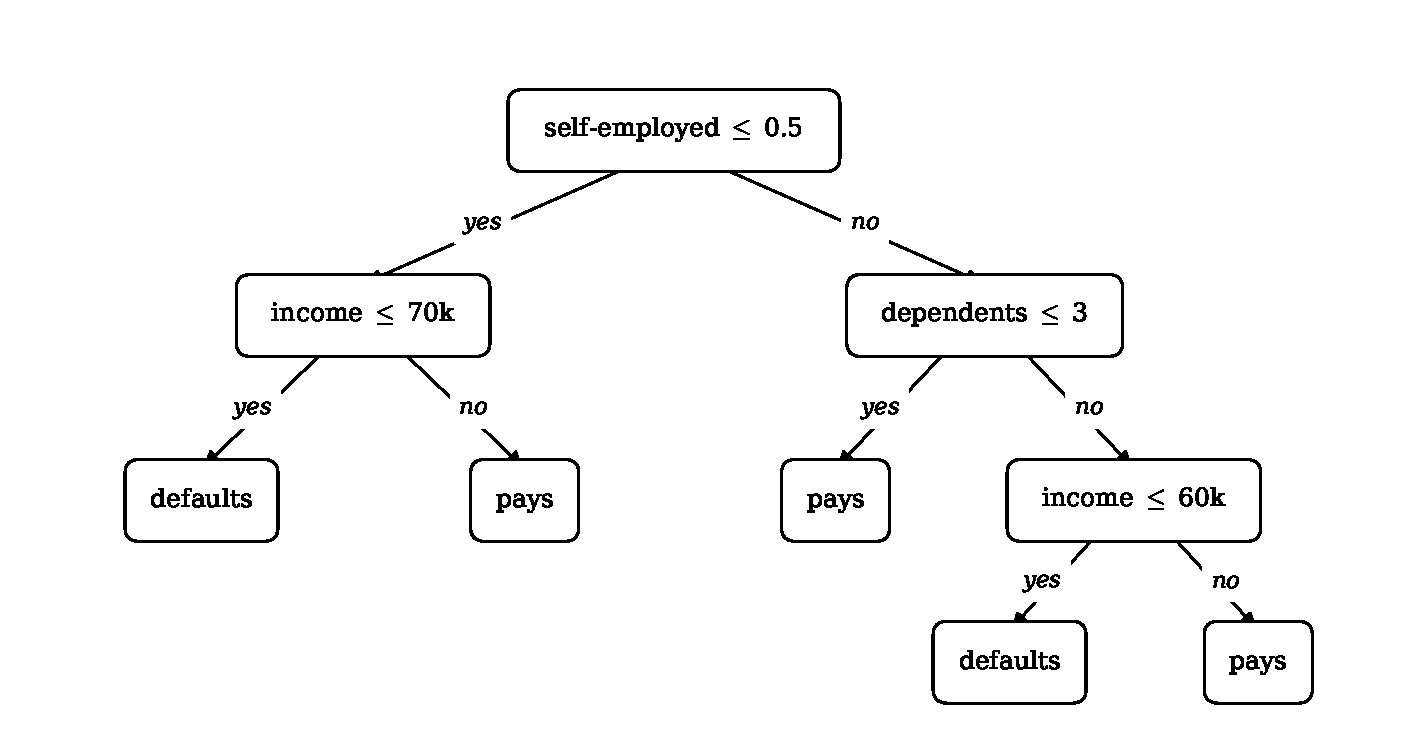
\includegraphics[width=\columnwidth]{forest_v2.pdf}
  \caption{A decision tree illustrating a loan approval problem, based on three features: self-employment (0 or 1), annual income, and the number of dependents. The nodes without conditions contain the prediction labels indicating whether the applicant would default or pay back the loan. For the underlying sample data, see Section \ref{sec:sample}.}
  \label{fig:dt}
\end{figure}

Ongoing research in the field continues to introduce new ideas: alternative impurity measures addressing biases of conventional ones \citep{dt-average-gain, dt-gain-minimum-entropy-of-error, dt-split-fuzzy, dt-split-rough-set}, multivariate/oblique splitting functions \citep{hhcart, dt-split-oblique-svm}, pruning techniques \citep{dt-pruning-evolutionary, dt-pruning-max-heap}, and applications beyond classic classification and regression, such as survival rate prediction \citep{survival-forest} and density estimation \citep{density-tree}. Further recent directions include tree learning with privacy \citep{privacy}, adaptation to big data \citep{bigdata}, and deep models \citep{decision-stream}. For further details, we refer to \citep{treebook, tutorial}.

Despite the numerous variants of decision tree learning proposed over the last decades, it is noteworthy that many applications, including those cited earlier, still rely on robust implementations of Classification and Regression Trees (CART) -- named, together with C4.5, among the most important algorithms in data mining \citep{top10} -- in the form of binary CART-type implementations (and their ensembles) available in packages such as \emph{sklearn} \citep{sklearn}, \emph{tree} \citep{tree}, \emph{caret} \citep{caret}, and WEKA \citep{weka}, commercial software like Matlab \citep{matlab} and Wolfram Mathematica \citep{mathematica}, and ensemble techniques such as random forests \citep{rf0}, xgboost \citep{xgboost}, and lightgbm \citep{lightgbm}. These implementations typically treat all features as continuous, and thus the partitioning of the training data and the feature space by thresholding conditions (such as the ones in Figure \ref{fig:dt}) is applied along all axes. However, in general, the partitioning of the finite amount of training data does not imply a unique partitioning of the continuous feature space. One ambiguity arises from the fact that if there are no observations for a feature between the observed $x^l$ and $x^u$ values, any threshold $t\in]x^l, x^u[$ leads to the same partitioning of training data. This ambiguity is usually resolved in alignment with the assumption of the features being continuous: if the threshold should fall between the observed $x^l$ and $x^u$ values, the mid-point $t=(x^l + x^u)/2$ is used, thus, assigning 50\% of the unlabeled interval to both the left and right partitions. Another ambiguity arises from the choice of conditioning: the Python implementation \emph{sklearn} \citep{sklearn} uses the operator $\leq$ in the form $x \leq t$, leading to partitions open from the left and closed from the right along each axis (as in Figure \ref{fig:dt}), however, the R implementation \emph{tree} \citep{tree} uses conditions of the form $x < t$. Considering the presumption of continuous features, the choice of conditioning operator should have a marginal effect, as a feature takes the exact value of a threshold with negligible probability. However, \emph{when a feature has values from a small and equidistant domain -- for example an integer-valued age or a monetary value rounded to whole units -- the thresholds determined as the mid-points of observations can coincide with feature values, making predictions dependent on the choice of conditioning operator and leading to a bias}.

Although it might seem to have a marginal effect, due to the popularity and numerous applications of binary decision trees and random forests, we dedicate this paper to investigating this potential bias, and to a careful treatment of how such a small effect can and cannot be legitimately demonstrated.
The contributions of the paper to the field can be summarized as follows:
\begin{enumerate}
\item We introduce the term \emph{conditioning bias} for the variation in predictions caused by the choice of conditioning operator, and demonstrate it mechanistically in decision trees and random forests with small, equidistant-domain features.
\item We propose practical bias-elimination techniques for both accessible and inaccessible tree internals, and show, with direct measurement, why bootstrap aggregation does \emph{not} average the bias away.
\item Through extensive, statistically rigorous testing on both real and synthetic data, we show that no individual operator is reliably better than the other, while the proposed averaging method robustly outperforms the worse-performing one.
\item We further show that cross-validating the operator choice does not outperform averaging or identify the better operator above chance, and that restricting evaluation to affected records only strengthens this conclusion.
\item Eliminating the bias in random forests costs nothing in training or inference time; since the bias itself is heavy-tailed and its severity cannot be known in advance, this makes the proposed method a \emph{free-lunch} safeguard worth adopting unconditionally.
\end{enumerate}
The proposed techniques and the completely reproducible implementation of the study, written in Python, are shared with the community in the GitHub repository \url{https://github.com/gykovacs/conditioning_bias}.

The paper is organized as follows: In Section \ref{sec:problem}, we formulate the problem and demonstrate its existence qualitatively. Section \ref{sec:proposed} describes the proposed solutions. The experimental setup and the results of the tests are presented and discussed in Section \ref{sec:tests}, and finally, conclusions are drawn in Section \ref{sec:summary}.

\section{Problem Formulation}
\label{sec:problem}

In this section, we provide an introduction to decision tree learning (subsections \ref{sec:problem-intro} and \ref{sec:problem-split}), and formulate the problem we address (subsection \ref{sec:problem-bias}).
Normal, boldface and calligraphic typesetting denote scalars (for example, $d \in\mathbb{Z}$), vectors (for example, $\mathbf{x}\in\mathbb{Z}^d$) and sets (for example, $\mathcal{S}\subset\mathbb{Z}$), respectively. Elements of sequences and sets are indexed by superscripts, coordinates of vectors are referred by subscripts.
We say that a feature $f$ has an \emph{equidistant domain} if it takes values from a small set of possible values that are spaced at (or near) regular intervals, such as integer ages, counts, or monetary amounts rounded to whole units.

\subsection{Decision tree induction}
\label{sec:problem-intro}

CART-type binary decision trees \citep{cart}, as implemented in the packages considered in this paper, treat all features as continuous and are built by recursively partitioning the training set, splitting each node on the feature $f$ and threshold $t$ that jointly minimize the impurity of the labels in the resulting left ($\mathbf{x}_f \leq t$) and right partitions. Since no training values fall inside the interval bounding an optimal split, most implementations set $t$ to its mid-point, symmetrically assigning half of the interval to each side. A direct consequence is that \emph{the choice of conditioning ($<$ or $\leq$) does not affect the tree induction itself}, only prediction, as discussed next. For a general treatment of decision tree induction, we refer to \citep{treebook}.

\subsection{Prediction with decision trees}
\label{sec:problem-split}

Prediction for a vector $\mathbf{x}$ is conducted by starting from the root node and recursively applying the condition $\mathbf{x}_{f} \leq t$ or $\mathbf{x}_{f} < t$, with the parameters $f$ and $t$ recorded in the current node, and routing $\mathbf{x}$ to the subtree corresponding to the output of the condition. Upon encountering a leaf node, the recorded statistics -- the class distribution, or its majority vote, for classification, and the mean target value for regression -- are returned as the prediction for $\mathbf{x}$.
The conditioning $\mathbf{x}_f\leq t$ aligns with the Python implementation \emph{sklearn} \citep{sklearn}, while other implementations (such as the R package \emph{caret} \citep{caret}) use conditions of the form $\mathbf{x}_{f} < t$.

Unlike tree induction, \emph{prediction can depend on the choice of conditioning operator}. Particularly, when a feature value coincides with a threshold, the routing of the vector depends on the conditioning.
For example, in the tree in Figure \ref{fig:dt}, there is a split on the attribute \emph{dependents} at 3, which can occur if the training set at the root node does not contain records with 3 dependents. The routing of records with $dependents=3$ (and, in this example, $self\text{-}employed=1$, so that the \emph{dependents} node is actually reached) is determined by the conditioning: with $\leq$ it is routed to the left and with $<$ to the right.

Naturally, with truly continuous features, the probability of a feature value matching a threshold is negligible. However, under the following circumstances, feature values can coincide with thresholds:
\begin{enumerate}
\item \emph{A feature has an equidistant domain with non-negligible probability}: the thresholds (mid-points) between observations being an even number of equidistant steps apart are also domain values.
\item \emph{Relatively deep trees are built}: a threshold can fall on a domain value only if it is missing from the training set at the respective node -- the deeper a tree gets, the smaller the training set becomes, leading to gaps in the representation of the feature domain.
\end{enumerate}
We highlight that features with equidistant domains are common in practice. For instance, the \emph{age} attribute in medical datasets; \emph{rounded decimals} when features are observed to a certain number of digits; and \emph{monetary values} quoted in units of millions in financial datasets to mention a few.
We also mention that due to the regularizing effect of bootstrap aggregation, the decision trees used in random forests need less regularization by depth, consequently, random forests can be expected to be more affected by the phenomenon; we return to this point, with direct empirical evidence, in Section \ref{sec:integrate}.

\subsection{The conditioning bias}
\label{sec:problem-bias}

It can be argued that the variation of predictions is due to using the mid-points as thresholds. However, the mid-points are reasonable choices for continuous features, any alternative would lead to asymmetries and consequent biases. Therefore, we consider the phenomenon to be \emph{an artifact of dealing with discrete features in a continuous framework}, and attribute it to the inadequacy of both conditioning operators in such cases.

For the ease of discussion, we introduce the term \emph{conditioning bias} to refer to the variation of predictions due to the choice of conditioning: for a fixed fitted tree, the prediction of a given $\mathbf{x}$ can differ depending only on whether $\leq$ or $<$ is used at prediction time, and this variation is what we refer to as the bias throughout the paper.
In the rest of the paper, we address the mitigation of the conditioning bias from the theoretical and practical points of view.

\section{The Proposed Method}
\label{sec:proposed}

This section introduces methods to mitigate the conditioning bias. Subsection \ref{sec:hyper} argues that \emph{the conditioning operator should not be treated as a hyperparameter}; subsection \ref{sec:integrate} proposes eliminating its detrimental effects by predicting with both operators and averaging the results. Since most implementations expose only one default conditioning form -- a constraint most acute in managed environments like Matlab \citep{matlab}, SAS \citep{sas}, and no-code platforms \citep{nocode} -- subsection \ref{sec:equiv} presents ways to obtain predictions under the non-default operator without modifying the inference engine.

\subsection{The conditioning operator as a hyperparameter}
\label{sec:hyper}

The conditioning operator could, in principle, be treated as another hyperparameter of tree induction, akin to maximum depth: one could assess both operators ($<$ and $\leq$) in a cross-validation scheme and select whichever performs better -- even per affected feature, or per affected node.

Unfortunately, proper cross-validation of the operator is not straightforward. Unlike genuine regularization parameters such as maximum depth or leaf size, which offer interpretable control over smoothness, conditioning affects only specific edge cases in unpredictable ways. In a typical (possibly iterated) cross-validation scheme, some percentage of the data is held out for testing; the two operators disagree on a test record only where a test feature value happens to coincide with a threshold along its decision path. But once the final model is refit on the full dataset, those particular coincidences vanish -- the very test records that produced them are now part of training -- while other thresholds, along other paths, can newly coincide with other domain values. The cross-validated comparison therefore has no reason to generalize: \emph{the difference in cross-validated performance between operators cannot be assumed to carry over to the model fitted on the full dataset}.

Direct evidence corroborates this concern. Our cross-dataset meta-analysis (Section \ref{sec:meta}) finds that across 40 datasets, a sign test on which operator wins per dataset never rejects a 50/50 split -- there is no consistent population-level winner to select for -- and an independent synthetic experiment with known ground truth (Section \ref{sec:synthetic}) reaches the same conclusion under a scheme needing no cross-validation correction at all. Cross-validating the operator would therefore typically tune to noise rather than signal, a conclusion Section \ref{sec:select} corroborates further by implementing such a selection procedure directly, with a proper nested design, and showing it fails to outperform simple averaging. Popular implementations already make this choice implicitly via their default operator, with no reason to expect better than 50\% odds of it being the right one when equidistant-domain features are present. We therefore focus not on selecting an operator, but on eliminating the downside risk of picking the wrong one, by integrating out the choice altogether.

\subsection{Integrating out the conditioning}
\label{sec:integrate}

A conservative approach to mitigating the conditioning bias is to integrate out the ambiguity: predicting with both operators and averaging the results eliminates the dependence on which one is used. Section \ref{sec:tests} validates this empirically, showing a statistically robust improvement, across the dataset pool, over whichever operator turns out to perform worse. The mechanism is variance reduction, not bias correction, in the classic sense: for a fixed tree and affected instance, the distortion is deterministic, not random, so averaging cannot correct it for that instance -- instead, it hedges against not knowing, in advance, which operator the distortion happens to favor.

For single decision trees, averaging both operators' predictions is straightforward: for classification, this means averaging the \emph{predicted class-probability distributions}, not taking a hard vote, so no tie-breaking rule is needed even when the operators would otherwise disagree on the predicted class. Computationally, this only doubles prediction time -- a favorable trade-off wherever execution time is not critical, and one that leaves decision trees competitive even so, given how fast they already are relative to techniques such as kNN.
Interpretability is a separate concern, since single trees are valued for the decision paths predictions traverse. When the two operators agree on the path (the usual case), interpretability is unaffected; when they diverge, both paths are equally valid, and reporting both is more honest than picking one, since relying on a single path would be just as misleading as the biased prediction it represents. A coin-flip tie-break would preserve a single path, but we do not pursue it: it forfeits averaging's variance-reduction benefit and, unlike averaging, does not extend to a free-lunch improvement for random forests (see below).

For random forests, the same approach applied to every tree would again double prediction time. But given the typically large ensemble size, evaluating half the trees with each operator gives a reasonably accurate approximation at no extra prediction cost -- making bias elimination a \emph{free lunch} for random forests.

It is natural to ask why bagging across a forest's many trees does not already average the bias away -- a question we answer with measurement, not argument alone. First, the conditioning operator is a constant, deterministic choice applied identically to every tree by the same implementation; it is not an independent, zero-mean source of variation across ensemble members for bagging to cancel, since bagging reduces \emph{variance across trees}, not a systematic choice shared by all of them. Second, individual forest trees are, on average, at least as susceptible to the bias as single decision trees under the same model-selection procedure, and somewhat more so: the proportion of nodes whose threshold coincides with an observed domain value ($\rho$, Section \ref{sec:tests-quant}) is, on average, 1.07--1.38 times higher in forest trees (0.145 vs.\ 0.200 for classification, 0.166 vs.\ 0.177 for regression), consistent with the lighter depth regularization bagging affords (Section \ref{sec:problem-split}). The margin is modest -- a single shared regularizing hyperparameter (maximum depth, Section \ref{sec:tests-model}) limits how differently the two are regularized -- but the direction is consistent, and bagging has no mechanism to cancel a deterministic property shared by every tree in the ensemble.

\subsection{Prediction with the non-default conditioning operator}
\label{sec:equiv}

Our proposed methods require predictions under both conditioning operators, yet popular implementations treat the operator as a fixed, unchangeable property. Since induction itself is unaffected by the operator but must remain efficient and typically involves advanced operations like pruning \citep{sklearn}, building custom implementations that expose the operator as a parameter is impractical, particularly in graphical and low/no-code environments \citep{nocode}. This subsection instead discusses alternative ways to obtain predictions under the non-default operator.

Let $\mathcal{T} = (\mathbf{x}_i, y_i)_{i=1}^N$ be a training set and $T_{\mathcal{T}}$ a tree fitted to it; without loss of generality, suppose the implementation intrinsically uses $\leq$, giving prediction $T_{\mathcal{T}}(\mathbf{x}, \leq)$. We seek the prediction under the non-default operator, $T_{\mathcal{T}}(\mathbf{x}, <)$ -- concretely, prediction with the tree in Figure \ref{fig:dt2-a}, given only the ability to predict with the tree in Figure \ref{fig:dt}.

Our workaround rests on the identity $\mathbf{x}_f < t \Leftrightarrow -\mathbf{x}_f \leq -t$: a vector routed left by $\mathbf{x}_f < t$ is routed right by $-\mathbf{x}_f \leq -t$. This motivates \emph{tree mirroring}, $\mathcal{M}[T_{\mathcal{T}}]$: recursively swapping each node's left and right subtrees and negating its threshold throughout the tree. Predicting the negated vector $-\mathbf{x}$ with the mirrored tree then reproduces, along the same (mirrored) decision path, the prediction that $\mathbf{x}$ would get from the original tree under the opposite operator: $T_{\mathcal{T}}(\mathbf{x}, <) = \mathcal{M}[T_{\mathcal{T}}](-\mathbf{x}, \leq)$.
Figure \ref{fig:dt2-b} plots the mirrored version of the tree in Figure \ref{fig:dt}. For $\mathbf{x} = (\text{self-employed}: 1, \text{dependents}: 3, \text{income}: 50k)$, a feature value that coincides with a threshold, the original tree and its non-default-operator counterpart (Figure \ref{fig:dt2-a}) disagree (\emph{pays} vs.\ \emph{defaults}); predicting $-\mathbf{x}$ with the mirrored tree (Figure \ref{fig:dt2-b}) reproduces the operator-$<$ result (\emph{defaults}), confirming the equivalence.

Depending on the accessibility of the trained tree structure, this equivalence yields two ways to obtain $T_{\mathcal{T}}(\mathbf{x}, <)$ without reimplementing prediction:
\begin{enumerate}
\item If \emph{the trained tree structure is accessible} (e.g., \emph{sklearn}'s \citep{sklearn} mutable tree structure), mirror it directly -- swap child nodes and negate thresholds -- then predict $-\mathbf{x}$ on the mirrored tree. This requires only a single traversal of the existing tree, cheaper than retraining.
\item If \emph{the trained tree structure is not accessible}, induce the mirrored tree directly from the negated training set $\mathcal{T}' = (-\mathbf{x}_i, y_i)_{i=1}^N$ and predict $-\mathbf{x}$ on it; equivalence again holds, up to any randomized tie-breaking between equally good splits during induction. This requires retraining, but works even in low/no-code environments \citep{nocode} where tree internals are inaccessible.
\end{enumerate}
These workarounds make it possible to compare and mitigate the effect of both conditioning operators in most machine learning environments without implementing custom prediction engines.

\begin{figure}[tbp]
  \centering
    \subfigure[\label{fig:dt2-a}]{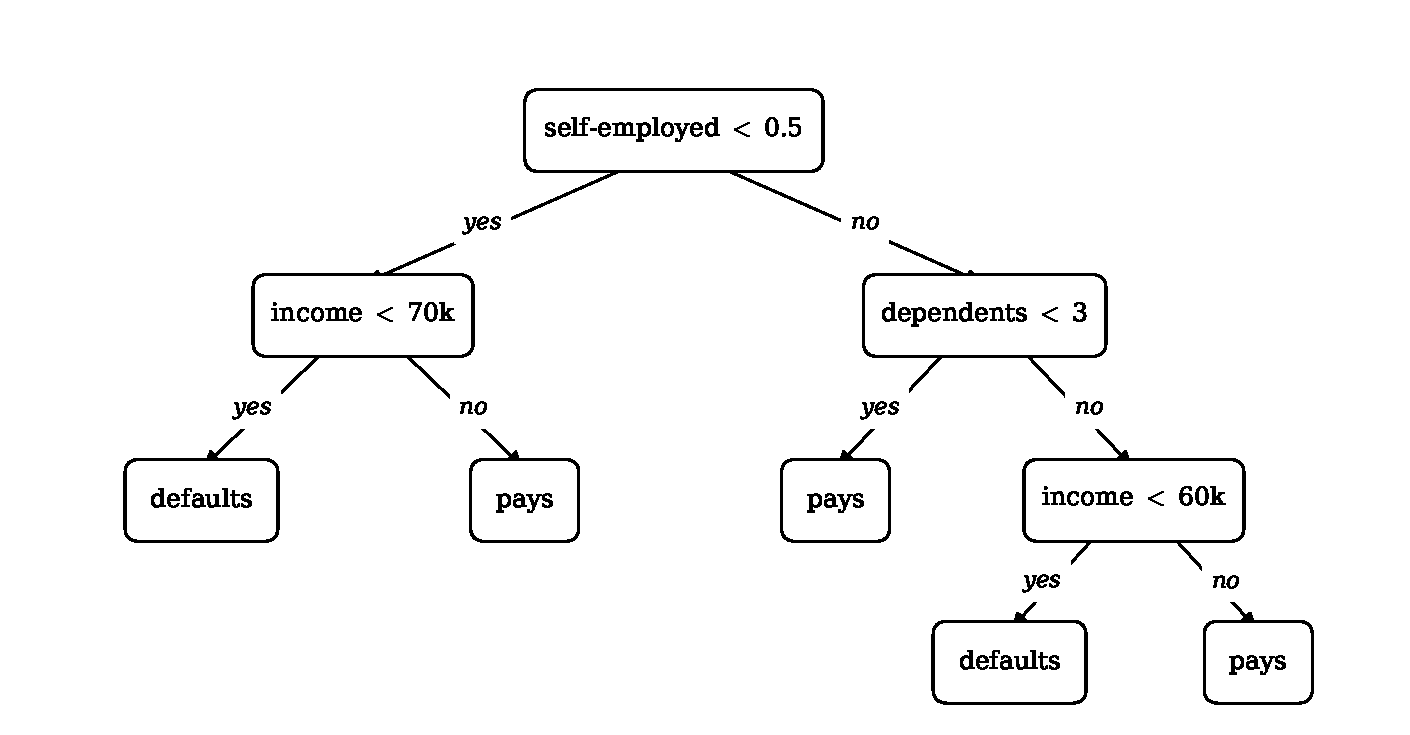
\includegraphics[width=0.85\columnwidth]{forest3_v2.pdf}}
    \subfigure[\label{fig:dt2-b}]{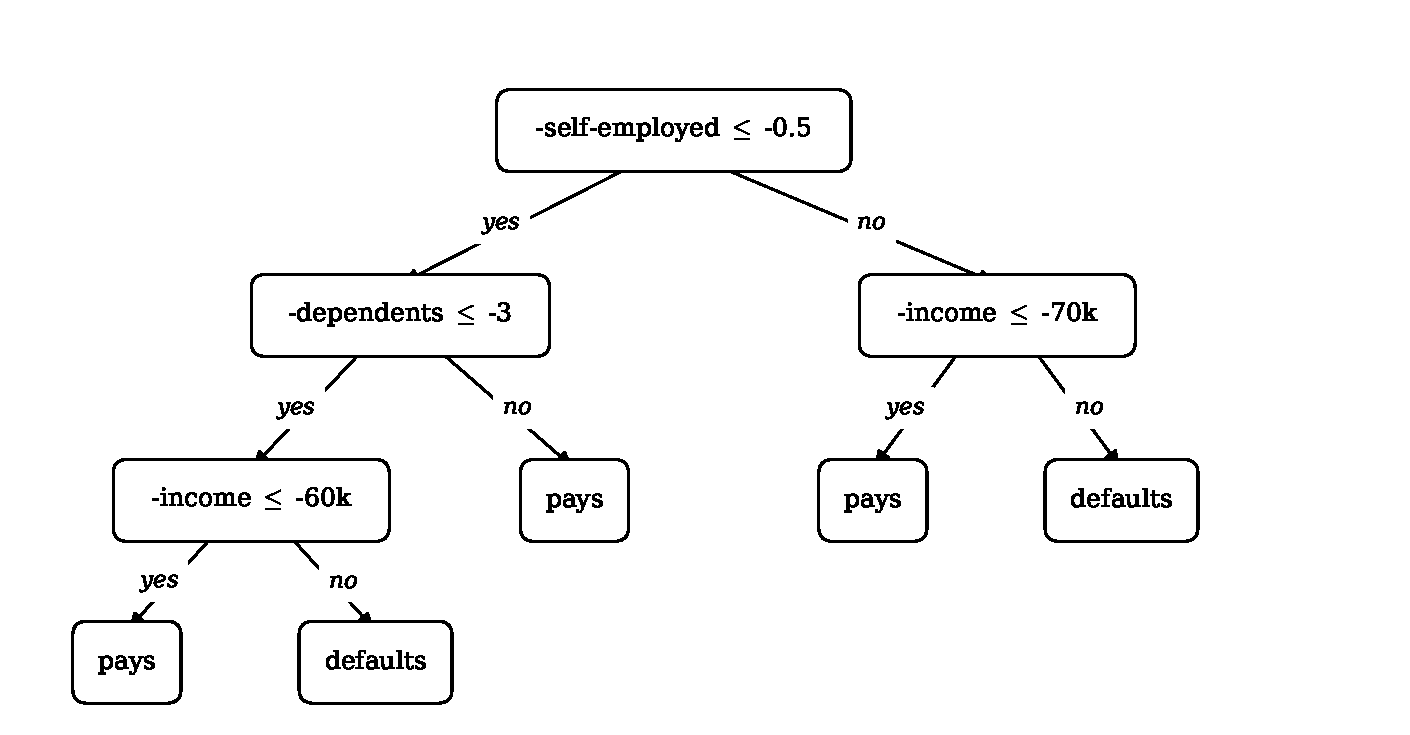
\includegraphics[width=0.85\columnwidth]{forest2_v2.pdf}}
  \caption{The decision tree in Figure \ref{fig:dt} with replaced conditioning operators (a), and its mirrored variant (b). One can check that given any feature vector $\mathbf{x}$, the prediction of $\mathbf{x}$ with (a) and that of $-\mathbf{x}$ with (b) leads to the same result along the same (but mirrored) decision path.}
  \label{fig:dt2}
\end{figure}

\section{Tests and Results}
\label{sec:tests}

In Section \ref{sec:problem}, we argued the conditioning bias can emerge in CART-type trees when features have equidistant domains; Section \ref{sec:proposed} introduced methods to mitigate it. This section (a) demonstrates the bias mechanistically, (b) establishes, with statistically valid testing, what can and cannot be claimed about operator performance, and (c) shows the proposed averaging method robustly reduces the risk of performance deterioration; we deemed comparisons to other state-of-the-art techniques unnecessary, given our focus on this specific characteristic of decision tree learning. A recurring pitfall in this kind of evaluation is treating the folds of repeated cross-validation or holdout as independent observations in a significance test, which is anti-conservative; Section \ref{sec:tests-testing} documents this and introduces the corrected test used throughout. Subsection \ref{sec:tests-methodology} lays out this methodology before any results are shown; Subsection \ref{sec:synthetic} applies it under an idealized, known ground truth to establish our central hypothesis -- no operator is reliably better, while averaging robustly outperforms the worse one; Subsection \ref{sec:real-data} then tests whether this hypothesis survives contact with real, finite datasets, where the correction is actually needed.

\subsection{Evaluation methodology}
\label{sec:tests-methodology}

\subsubsection{The role of cross-validation}
\label{sec:tests-cv}

In subsection \ref{sec:hyper}, we discussed why cross-validation cannot be used to select the conditioning operator with the intention of then fitting a single final model to all available data and expecting the selection to carry over. This is a statement about the target of selection -- a single conditioning choice meant to generalize to the fully-refit model -- not about whether cross-validation can be trusted at all. Cross-validation remains entirely valid, and is what we use throughout Section \ref{sec:tests}, for two related but distinct purposes: quantitatively estimating the magnitude of the bias and the relative performance of the two operators on genuinely held-out data (Sections \ref{sec:tests-quant}--\ref{sec:tests-proposed}), and, separately, evaluating whether a per-split, freshly re-selected choice of operator -- one that never claims to generalize beyond the split it was chosen on -- is a competitive alternative to averaging (Section \ref{sec:select}). The nested design of Section \ref{sec:tests-model}, in which every hyperparameter and operator selection is confined to the training portion of its own evaluation split, is what makes the latter a fair comparison rather than the kind of leakage discussed above.


\subsubsection{Model and operator selection}
\label{sec:tests-model}

For realistic evaluations, selecting appropriate hyperparameters is crucial: shallow trees rarely exhibit the conditioning bias, while unconstrained trees exaggerate it but are highly overfit.

We regularize trees and forests using a single hyperparameter, the \emph{maximum depth} $\beta \in \{2,\dots,15,\infty\}$ ($\infty$ denoting an unconstrained tree) -- a deliberately simple choice that keeps fully nested selection of both the hyperparameter and the conditioning operator, independently for every evaluation split, computationally practical at the scale of this study (40 datasets $\times$ 4 estimator types $\times$ 100 repeated splits).

Within the training portion of each of the $R=100$ outer evaluation splits (Section \ref{sec:tests-testing}), an inner 5-fold cross-validation (i) selects $\beta$ by scoring every candidate depth against the default operator, then (ii) scores $\leq$ against $<$ at the selected $\beta$ and picks whichever scored higher -- both on the same inner validation folds. The model is then refit once, at the selected $\beta$, on the full training portion, and $\leq$, $<$, the average, and the selected operator are all evaluated on the outer split's held-out test portion, untouched by either selection.

As anticipated, the regularization of decision trees is more pronounced compared to random forests, with optimal performance typically achieved using a smaller maximum depth. When the trees are extremely shallow ($\beta \leq 3$), as is often the case in decision tree classification, the impact of the conditioning bias is expected to be less significant.


\subsubsection{Hypothesis testing}
\label{sec:tests-testing}

We are set to investigate a presumably small effect, which places unusual demands on how significance is tested.

A common but flawed practice is to pool cross-validation fold scores across repeats and treat them as independent observations in a paired significance test; because folds overlap by construction, this is anti-conservative, routinely reporting $p$-values orders of magnitude too small \citep{dietterich1998, nadeau2003, bengio2004}. We avoid this throughout using the corrected resampled $t$-test described next.

We use the corrected resampled $t$-test of Nadeau and Bengio \citeyearpar{nadeau2003}, later adapted by Bouckaert and Frank \citeyearpar{bouckaert2004} to the $K$-fold case: its variance correction depends on the train/test size ratio and does not shrink with the number of repeats, so \emph{beyond a moderate number of repeats, additional repetitions buy diminishing statistical power} -- the only way to meaningfully increase power is to raise $K$ (or, for holdout, the training fraction $p$).

This is what determines the evaluation design used from Section \ref{sec:tests-quant} onward. We use repeated random holdout (via \texttt{ShuffleSplit}/\texttt{StratifiedShuffleSplit}) at a training fraction $p=0.9$, matching the correction floor of $10$-fold cross-validation -- large enough to keep the floor modest, while still leaving each split's training portion close to the size of the full dataset, which matters both for the smaller datasets in the pool and for the nested selection procedure of Section \ref{sec:tests-model}. We use $R=100$ repeated splits throughout, well past the point of diminishing returns from additional repeats.

\subsection{Synthetic validation}
\label{sec:synthetic}

\subsubsection{Data-generating process and protocol}

Before turning to real, finite datasets and the statistical machinery that repeated resampling on them requires, we first establish our central two-part hypothesis under an idealized setting with a known, controllable ground truth: a synthetic data-generating process with a controllable discrete/equidistant feature (domain size and step configurable) alongside continuous filler features, applied to all four estimator/problem-type combinations used elsewhere in the paper. This check deliberately targets only that central hypothesis; the two further questions addressed on real data below -- whether cross-validation can select the operator directly (Section \ref{sec:select}) and how the bias concentrates on individual affected records (Section \ref{sec:biased-instances}) -- depend on nested cross-validation and per-instance analysis machinery that would be circular to apply to data whose ground truth is already known by construction.

Because the generating process is known, we can draw a fresh, independent and identically distributed test set for every replicate, sidestepping the repeated-CV non-independence issue entirely rather than correcting for it: for each of $R=100$ independent replicates per configuration, we drew a fresh training set ($500$ records), fit the model once with a fixed hyperparameter, and scored $\leq$, $<$, and the proposed average on a fresh $50{,}000$-record test set. The resulting $100$ per-replicate score differences are genuinely independent, so an ordinary Wilcoxon signed-rank test is valid without any correction. We swept two knobs known to control whether the bias can manifest at all (Section \ref{sec:problem-split}): the granularity of the discrete feature's domain (domain sizes $\{5,11,21,51\}$, at a fixed depth of $8$) and the maximum tree depth ($\{3,5,8,12\}$, at a fixed domain size of $11$), giving $8$ configurations for each of the four estimator/problem-type combinations.


\subsubsection{No individual operator is reliably better}

We first test the first half of our central hypothesis under this idealized scheme: whether either conditioning operator is reliably better than the other across the swept configurations.

\begin{table*}[tbp]
  \caption{Synthetic validation, $\leq$ vs.\ $<$: for each of $32$ (estimator $\times$ configuration) combinations, the absolute mean scores ($s_{\leq}$, $s_{<}$), their difference (\emph{diff}), and the Wilcoxon $p$-value, with $\ast$ marking $p<0.05$. Replicate scores are genuinely independent by construction (fresh i.i.d.\ test data per replicate), so no cross-validation correction is needed or applied.}
  \label{tab:synthetic-null}
  \centering
    \begin{footnotesize}
      \begin{tabular}{l@{\hspace{6pt}}r@{\hspace{5pt}}r@{\hspace{5pt}}r@{\hspace{5pt}}r@{\hspace{5pt}}c@{\hspace{10pt}}r@{\hspace{5pt}}r@{\hspace{5pt}}r@{\hspace{5pt}}r@{\hspace{5pt}}c@{\hspace{10pt}}r@{\hspace{5pt}}r@{\hspace{5pt}}r@{\hspace{5pt}}r@{\hspace{5pt}}c@{\hspace{10pt}}r@{\hspace{5pt}}r@{\hspace{5pt}}r@{\hspace{5pt}}r@{\hspace{5pt}}c}
\toprule
& \multicolumn{5}{c}{DT classif.} & \multicolumn{5}{c}{RF classif.} & \multicolumn{5}{c}{DT regr.} & \multicolumn{5}{c}{RF regr.} \\
value & $s_{\leq}$ & $s_{<}$ & diff & $p$ &  & $s_{\leq}$ & $s_{<}$ & diff & $p$ &  & $s_{\leq}$ & $s_{<}$ & diff & $p$ &  & $s_{\leq}$ & $s_{<}$ & diff & $p$ &  \\
\midrule
\multicolumn{21}{l}{\emph{Domain-size sweep (max depth fixed at 8)}} \\
5 & 0.846 & 0.846 & 1.3e-04 & 1.5e-01 &  & 0.961 & 0.961 & 1.1e-05 & 5.4e-01 &  & 0.740 & 0.740 & 9.3e-05 & 7.2e-01 &  & 0.876 & 0.876 & 8.3e-06 & 8.6e-01 &  \\
11 & 0.900 & 0.900 & 1.0e-04 & 3.9e-01 &  & 0.984 & 0.984 & -1.3e-05 & 7.4e-01 &  & 0.863 & 0.863 & 6.7e-05 & 8.3e-01 &  & 0.938 & 0.938 & 2.9e-06 & 8.4e-01 &  \\
21 & 0.941 & 0.941 & 6.9e-05 & 9.2e-01 &  & 0.993 & 0.993 & -1.1e-05 & 9.9e-01 &  & 0.943 & 0.943 & 1.3e-05 & 4.5e-01 &  & 0.975 & 0.975 & -3.9e-06 & 6.7e-01 &  \\
51 & 0.972 & 0.972 & 2.2e-05 & 2.9e-01 &  & 0.998 & 0.998 & 2.3e-05 & 3.2e-01 &  & 0.986 & 0.986 & -1.6e-06 & 4.3e-01 &  & 0.993 & 0.993 & -1.1e-05 & 4.9e-03 & $\ast$ \\
\midrule
\multicolumn{21}{l}{\emph{Depth sweep (domain size fixed at 11)}} \\
3 & 0.924 & 0.924 & -7.2e-05 & 7.0e-01 &  & 0.973 & 0.973 & -2.4e-08 & 4.0e-01 &  & 0.744 & 0.744 & 0 & 1 &  & 0.819 & 0.819 & 0 & 1 &  \\
5 & 0.921 & 0.921 & 1.1e-05 & 7.6e-01 &  & 0.981 & 0.981 & 1.7e-05 & 3.9e-01 &  & 0.819 & 0.819 & -1.1e-05 & 7.0e-01 &  & 0.904 & 0.904 & 5.6e-06 & 6.9e-01 &  \\
8 & 0.900 & 0.900 & 1.3e-04 & 3.0e-01 &  & 0.983 & 0.983 & 1.0e-05 & 5.8e-01 &  & 0.864 & 0.864 & 5.1e-05 & 6.3e-01 &  & 0.939 & 0.939 & -1.9e-05 & 1.0e-01 &  \\
12 & 0.897 & 0.897 & 3.2e-05 & 5.6e-01 &  & 0.983 & 0.983 & 4.8e-05 & 1.5e-02 & $\ast$ & 0.865 & 0.865 & -4.1e-05 & 2.6e-01 &  & 0.942 & 0.942 & -2.4e-06 & 7.1e-01 &  \\
\bottomrule
\end{tabular}

    \end{footnotesize}
\end{table*}

Table \ref{tab:synthetic-null} reports $\leq$ versus $<$ for every configuration: only $2$ of $32$ reach nominal significance at $p<0.05$ -- almost exactly the rate expected from chance alone under a true null across $32$ independent tests -- and even those two carry a negligible mean difference ($4.8\times10^{-5}$ and $-1.1\times10^{-5}$). Under this idealized testing scheme, with no cross-validation artifacts to correct for, no individual conditioning operator is reliably better than the other -- the first half of our central hypothesis, which we test again on real data in Section \ref{sec:meta}.

\subsubsection{The averaging method robustly outperforms the worse operator}

We now turn to the second half of our central hypothesis: whether the proposed averaging method robustly outperforms the worse-performing individual operator whenever the bias has an opportunity to manifest.

\begin{table*}[tbp]
  \caption{Synthetic validation, averaging vs.\ $\text{worst}(\leq,<)$: same format as Table \ref{tab:synthetic-null}, with absolute mean scores $s_{avg}$ and $s_{worst}$.}
  \label{tab:synthetic}
  \centering
    \begin{footnotesize}
      \begin{tabular}{l@{\hspace{6pt}}r@{\hspace{5pt}}r@{\hspace{5pt}}r@{\hspace{5pt}}r@{\hspace{5pt}}c@{\hspace{10pt}}r@{\hspace{5pt}}r@{\hspace{5pt}}r@{\hspace{5pt}}r@{\hspace{5pt}}c@{\hspace{10pt}}r@{\hspace{5pt}}r@{\hspace{5pt}}r@{\hspace{5pt}}r@{\hspace{5pt}}c@{\hspace{10pt}}r@{\hspace{5pt}}r@{\hspace{5pt}}r@{\hspace{5pt}}r@{\hspace{5pt}}c}
\toprule
& \multicolumn{5}{c}{DT classif.} & \multicolumn{5}{c}{RF classif.} & \multicolumn{5}{c}{DT regr.} & \multicolumn{5}{c}{RF regr.} \\
value & $s_{avg}$ & $s_{worst}$ & diff & $p$ &  & $s_{avg}$ & $s_{worst}$ & diff & $p$ &  & $s_{avg}$ & $s_{worst}$ & diff & $p$ &  & $s_{avg}$ & $s_{worst}$ & diff & $p$ &  \\
\midrule
\multicolumn{21}{l}{\emph{Domain-size sweep (max depth fixed at 8)}} \\
5 & 0.846 & 0.846 & 1.8e-04 & 7.0e-02 &  & 0.961 & 0.961 & 6.5e-05 & 1.3e-10 & $\ast$ & 0.740 & 0.740 & 1.9e-04 & 2.3e-06 & $\ast$ & 0.876 & 0.876 & 5.2e-05 & 1.9e-11 & $\ast$ \\
11 & 0.900 & 0.899 & 7.9e-04 & 4.1e-07 & $\ast$ & 0.984 & 0.984 & 1.0e-04 & 7.7e-14 & $\ast$ & 0.863 & 0.863 & 1.4e-04 & 2.3e-10 & $\ast$ & 0.938 & 0.938 & 4.0e-05 & 2.1e-13 & $\ast$ \\
21 & 0.941 & 0.941 & 3.6e-04 & 1.2e-05 & $\ast$ & 0.993 & 0.993 & 9.4e-05 & 2.2e-10 & $\ast$ & 0.943 & 0.943 & 7.0e-05 & 5.9e-15 & $\ast$ & 0.975 & 0.975 & 2.9e-05 & 1.5e-14 & $\ast$ \\
51 & 0.972 & 0.972 & 9.9e-05 & 3.3e-02 & $\ast$ & 0.998 & 0.998 & 1.3e-04 & 1.9e-14 & $\ast$ & 0.986 & 0.986 & 4.0e-05 & 2.9e-17 & $\ast$ & 0.993 & 0.993 & 1.5e-05 & 3.3e-15 & $\ast$ \\
\midrule
\multicolumn{21}{l}{\emph{Depth sweep (domain size fixed at 11)}} \\
3 & 0.924 & 0.924 & 5.8e-05 & 7.0e-01 &  & 0.973 & 0.973 & 4.5e-05 & 2.1e-08 & $\ast$ & 0.744 & 0.744 & 0 & 1 &  & 0.819 & 0.819 & 4.4e-18 & 5.0e-01 &  \\
5 & 0.921 & 0.921 & 4.3e-04 & 8.7e-04 & $\ast$ & 0.981 & 0.981 & 8.1e-05 & 1.4e-13 & $\ast$ & 0.819 & 0.819 & 1.0e-05 & 7.0e-01 &  & 0.904 & 0.904 & 1.4e-05 & 7.4e-07 & $\ast$ \\
8 & 0.900 & 0.900 & 5.4e-04 & 7.3e-07 & $\ast$ & 0.983 & 0.983 & 1.2e-04 & 3.2e-13 & $\ast$ & 0.864 & 0.864 & 1.4e-04 & 2.3e-13 & $\ast$ & 0.939 & 0.939 & 4.2e-05 & 3.8e-10 & $\ast$ \\
12 & 0.897 & 0.897 & 4.8e-04 & 4.1e-07 & $\ast$ & 0.983 & 0.983 & 1.0e-04 & 4.6e-14 & $\ast$ & 0.866 & 0.865 & 1.6e-04 & 6.2e-17 & $\ast$ & 0.942 & 0.942 & 4.2e-05 & 6.9e-12 & $\ast$ \\
\bottomrule
\end{tabular}

    \end{footnotesize}
\end{table*}

Table \ref{tab:synthetic} reports the averaging-method comparison for every configuration, and here the picture is the opposite: $27$ of $32$ configurations are significant, several at $p<10^{-14}$. The $5$ exceptions are concentrated exactly where the mechanistic argument of Section \ref{sec:problem-split} predicts they should be: decision tree classification, decision tree regression, and random forest regression all lose significance at the shallowest depth tested ($\text{depth}=3$; for decision tree regression the effect is exactly zero there, since no lattice-aligned threshold ever forms), and decision tree classification also loses it at the coarsest domain granularity tested ($\text{domain size}=5$). Random forest classification, by contrast, is significant at every single configuration tested, including depth $3$ -- consistent with the finding of Section \ref{sec:integrate} that random forest trees are, if anything, more susceptible to the bias than single decision trees fit under the same regularization. Under this idealized, correction-free testing scheme, then, the proposed averaging method robustly outperforms the worse-performing individual operator whenever the bias has any opportunity to manifest at all -- the second half of our central hypothesis. The remainder of this section now tests whether both halves of this hypothesis hold up on real, finite datasets, which require the careful statistical corrections introduced next.


\subsection{Real-data evaluation}
\label{sec:real-data}


\subsubsection{Datasets}
\label{sec:tests-datasets}

To facilitate the selection of datasets for testing and evaluation, we introduce a heuristic condition. We consider a feature susceptible to the conditioning bias if there exists an observed domain value $\mathbf{x}_f$ and a positive real number $r\in\mathbb{R}^+$ such that $\mathbf{x}_f-r$ or $\mathbf{x}_f+r$ is also observed. This condition ensures that at least one threshold might align with a domain value. It is worth noting that this condition is not necessary; previously unseen records can still interfere with thresholds, even if none of the features in the training data meet the condition.

We selected 20 binary classification and 20 regression datasets primarily from the UCI \citep{uci} and KEEL \citep{keel} repositories, using the criteria that each dataset should contain \emph{at least one feature susceptible to the conditioning bias} and have enough samples for meaningful 10-fold cross-validation, and ranking eligible datasets by their size ($N \times N_a$, the number of records times the number of attributes) to select the 20 smallest in each category. The dataset collection preceded all experiments and was not influenced by any experimental results.

\begin{table*}[tbp]
  \caption{A summary of the key characteristics of the datasets used for evaluation, with $N$, $N_a$ and $N_b$ representing the number of records, attributes and the number of attributes susceptible to the bias, respectively. The counts of attributes were determined after the encoding of categorical attributes. $N_m$ denotes the number of minority samples in classification problems. The datasets are sorted by their size $N\cdot N_a$. Unless noted otherwise, classification datasets are drawn from KEEL \citep{keel} (\emph{hepatitis} from \citep{krnn}); regression datasets are drawn from KEEL \citep{keel}, UCI \citep{uci}, or \citep{krnn}, except \emph{medical-cost} \citep{mlwithr} and \emph{boom-bikes} \citep{boombikes}.}
  \label{tab:datasets}
  \centering
    \begin{footnotesize}
      \begin{minipage}[t]{0.48\textwidth}
        \centering
        \begin{tabular}{l@{\hspace{16pt}}r@{\hspace{16pt}}r@{\hspace{16pt}}r@{\hspace{16pt}}r}
\toprule
\multicolumn{5}{c}{Classification} \\
dataset & N & $N_a$ & $N_b$ & $N_m$ \\
\midrule
appendicitis & 106 & 7 & 7 & 21 \\
haberman & 306 & 3 & 3 & 81 \\
new-thyroid1 & 215 & 5 & 5 & 35 \\
glass0 & 214 & 9 & 9 & 70 \\
shuttle-6-vs-2-3 & 230 & 9 & 9 & 10 \\
bupa & 345 & 6 & 6 & 145 \\
cleveland-0-vs-4 & 177 & 13 & 10 & 13 \\
ecoli1 & 336 & 7 & 5 & 77 \\
poker-9-vs-7 & 244 & 10 & 10 & 8 \\
monk-2 & 432 & 6 & 4 & 204 \\
hepatitis & 155 & 19 & 6 & 32 \\
yeast-0-3-5-9-vs-7-8 & 506 & 8 & 6 & 50 \\
mammographic & 830 & 5 & 5 & 403 \\
saheart & 462 & 9 & 8 & 160 \\
page-blocks-1-3-vs-4 & 472 & 10 & 10 & 28 \\
lymphography & 148 & 32 & 3 & 6 \\
pima & 768 & 8 & 8 & 268 \\
wisconsin & 683 & 9 & 9 & 239 \\
abalone9-18 & 731 & 9 & 7 & 42 \\
winequality-red-3-vs-5 & 691 & 11 & 11 & 10 \\
\bottomrule
\end{tabular}

      \end{minipage}
      \hfill
      \begin{minipage}[t]{0.48\textwidth}
        \centering
        \begin{tabular}{l@{\hspace{16pt}}r@{\hspace{16pt}}r@{\hspace{16pt}}r}
\toprule
\multicolumn{4}{c}{Regression} \\
dataset & N & $N_a$ & $N_b$ \\
\midrule
stock-portfolio & 63 & 6 & 6 \\
wsn-ale & 107 & 5 & 4 \\
daily-demand & 60 & 12 & 7 \\
slump-test & 103 & 9 & 9 \\
servo & 167 & 10 & 2 \\
yacht-hydrodynamics & 307 & 6 & 6 \\
autoMPG6 & 392 & 5 & 5 \\
excitation-current & 557 & 4 & 4 \\
real-estate-valuation & 414 & 6 & 5 \\
wankara & 321 & 9 & 9 \\
plastic & 1650 & 2 & 2 \\
laser & 993 & 4 & 4 \\
qsar-aquatic-toxicity & 546 & 8 & 8 \\
baseball & 337 & 16 & 12 \\
maternal-health-risk & 1013 & 6 & 6 \\
cpu-performance & 209 & 35 & 6 \\
airfoil & 1503 & 5 & 4 \\
medical-cost & 1338 & 6 & 2 \\
boom-bikes & 730 & 13 & 10 \\
concrete & 1030 & 8 & 8 \\
\bottomrule
\end{tabular}

      \end{minipage}
    \end{footnotesize}
\end{table*}

As observed in Table \ref{tab:datasets}, the datasets cover approximately an order of magnitude range in both the number of training records and the number of features. Interestingly, features susceptible to the bias are more frequent in commonly used evaluation datasets than we anticipated; in many cases, all features meet the condition, despite the requirement being to have at least one such feature. To further support the claim regarding the frequency of features susceptible to the bias, it is noteworthy that the average proportion of such features within the toy datasets available in the \emph{sklearn} \citep{sklearn} package is 97\% -- almost all features of all toy datasets belong to this category.

The same preprocessing steps were applied to all datasets. First, missing data imputation was performed using the most frequent value. Next, for categorical features with at most 5 categories, one-hot encoding was applied, while integer encoding was used for features with more than 5 categories. Standardization was not necessary when working with tree techniques. We note that the presence of the bias depends on the representativeness of features at certain nodes, rather than on the overall size of the training set. The bias can emerge even when a dataset consists of millions of records if sufficiently deep trees are induced.


\subsubsection{Quantitative illustration of the effect}
\label{sec:tests-quant}

In this subsection, we investigate the existence of the conditioning bias quantitatively, using decision tree and random forest classification and regression.

\begin{table*}[tbp]
  \caption{Presence of the bias and evaluation of the proposed method, using the corrected significance testing procedure of Section \ref{sec:tests-testing} (repeated holdout, $p=0.9$, $R=100$, equivalent to a $K=10$ correction floor). In each block (classification and regression, decision tree and random forest rows per dataset), the columns $\rho$ and $\rho_k$ indicate the proportion of nodes with thresholds on feature domain values when the model is fitted to all data and, on average, to the training portion of the evaluation splits, respectively. The columns $auc_{\leq}$/$auc_{<}$ (and $r^2_{\leq}$/$r^2_{<}$) report the absolute mean performance scores of the default and non-default operators, with $auc_d$/$r^2_d$ their difference and $\ast$ in $p_{\neq}$ indicating the corrected test rejects the equality of the two operators' mean scores ($p<0.05$). The columns $auc_{avg}$/$r^2_{avg}$ report the proposed averaging method's absolute mean score, with $\ast$ in $p_{avg}$ indicating a statistically significant difference from the worse-performing of the two individual operators (worst$(\leq, <)$).}
  \label{tab:proof}
  \centering
    \begin{footnotesize}
      \begin{minipage}[t]{0.49\textwidth}
        \centering
        \begin{tabular}{l@{\hspace{3pt}}r@{\hspace{3pt}}r@{\hspace{3pt}}r@{\hspace{3pt}}r@{\hspace{3pt}}r@{\hspace{3pt}}c@{\hspace{3pt}}r@{\hspace{3pt}}c}
\toprule
\multicolumn{9}{c}{Classification} \\
dataset & $\rho$ & $\rho_{k}$ & auc$_{\leq}$ & auc$_{<}$ & auc$_{d}$ & p$_{\neq}$ & auc$_{avg}$ & p$_{avg}$ \\
\midrule
\multicolumn{9}{l}{\emph{Decision Tree}} \\
appendicitis & 0 & .08 & 0.732 & 0.732 & 0 &  & 0.732 &  \\
haberman & .25 & .24 & 0.602 & 0.601 &  1e-03 &  & 0.602 &  \\
new-thyroid1 & 0 & .12 & 0.921 & 0.930 & -9e-03 &  & 0.930 &  \\
glass0 & .20 & .20 & 0.817 & 0.817 & 0 &  & 0.817 &  \\
shuttle-6-vs-2-3 & 0 & 0 & 1.000 & 1.000 & 0 &  & 1.000 &  \\
bupa & .27 & .26 & 0.660 & 0.657 &  2e-03 &  & 0.660 &  \\
cleveland-0-vs-4 & .25 & .15 & 0.722 & 0.722 &  3e-04 &  & 0.722 &  \\
ecoli1 & .19 & .28 & 0.946 & 0.946 & -5e-05 &  & 0.946 &  \\
poker-9-vs-7 & 0 & .15 & 0.635 & 0.636 & -1e-03 &  & 0.636 &  \\
monk-2 & 0 & 0 & 1.000 & 1.000 & 0 &  & 1.000 &  \\
hepatitis & .21 & .11 & 0.654 & 0.654 & 0 &  & 0.654 &  \\
yeast-0-3-5-9-vs-7-8 & .30 & .28 & 0.693 & 0.693 & 0 &  & 0.693 &  \\
mammographic & .13 & .13 & 0.881 & 0.883 & -2e-03 &  & 0.883 &  \\
saheart & .25 & .19 & 0.692 & 0.691 &  8e-04 &  & 0.692 &  \\
page-blocks-1-3-vs-4 & 0 & .04 & 0.955 & 0.955 & 0 &  & 0.955 &  \\
lymphography & 0 & 0 & 0.886 & 0.890 & -4e-03 &  & 0.890 &  \\
pima & .30 & .30 & 0.778 & 0.777 &  1e-03 &  & 0.778 &  \\
wisconsin & .16 & .20 & 0.959 & 0.959 & -9e-06 &  & 0.960 &  \\
abalone9-18 & .17 & .16 & 0.658 & 0.658 & 0 &  & 0.658 &  \\
winequality-red-3-vs-5 & .20 & .20 & 0.517 & 0.517 & 0 &  & 0.517 &  \\
\midrule
\multicolumn{9}{l}{\emph{Random Forest}} \\
appendicitis & .13 & .09 & 0.851 & 0.851 & -6e-04 &  & 0.851 &  \\
haberman & .28 & .27 & 0.686 & 0.686 &  7e-04 &  & 0.686 &  \\
new-thyroid1 & .25 & .25 & 1.000 & 1.000 & 0 &  & 1.000 &  \\
glass0 & .22 & .19 & 0.944 & 0.944 & 0 &  & 0.944 &  \\
shuttle-6-vs-2-3 & .14 & .13 & 1.000 & 1.000 & 0 &  & 1.000 &  \\
bupa & .30 & .30 & 0.762 & 0.761 &  8e-04 &  & 0.763 & $\ast$ \\
cleveland-0-vs-4 & .19 & .20 & 0.980 & 0.980 & -3e-04 &  & 0.981 &  \\
ecoli1 & .33 & .32 & 0.957 & 0.957 & -2e-04 &  & 0.957 &  \\
poker-9-vs-7 & .16 & .18 & 0.989 & 0.990 & -2e-03 &  & 0.989 &  \\
monk-2 & .04 & .06 & 1.000 & 1.000 & 0 &  & 1.000 &  \\
hepatitis & .15 & .14 & 0.874 & 0.874 & -5e-04 &  & 0.875 &  \\
yeast-0-3-5-9-vs-7-8 & .28 & .29 & 0.799 & 0.800 & -1e-03 &  & 0.800 &  \\
mammographic & .19 & .19 & 0.916 & 0.916 &  3e-06 &  & 0.916 &  \\
saheart & .22 & .21 & 0.761 & 0.762 & -5e-04 &  & 0.761 &  \\
page-blocks-1-3-vs-4 & .09 & .07 & 0.999 & 0.999 & 0 &  & 0.999 &  \\
lymphography & .04 & .04 & 0.994 & 0.996 & -2e-03 &  & 0.996 &  \\
pima & .33 & .32 & 0.831 & 0.831 & -2e-04 &  & 0.830 &  \\
wisconsin & .21 & .21 & 0.993 & 0.993 & -4e-04 &  & 0.993 &  \\
abalone9-18 & .19 & .18 & 0.834 & 0.834 &  2e-04 &  & 0.834 &  \\
winequality-red-3-vs-5 & .25 & .26 & 0.834 & 0.833 &  5e-04 &  & 0.834 &  \\
\bottomrule
\end{tabular}

      \end{minipage}
      \hfill
      \begin{minipage}[t]{0.49\textwidth}
        \centering
        \begin{tabular}{l@{\hspace{3pt}}r@{\hspace{3pt}}r@{\hspace{3pt}}r@{\hspace{3pt}}r@{\hspace{3pt}}r@{\hspace{3pt}}c@{\hspace{3pt}}r@{\hspace{3pt}}c}
\toprule
\multicolumn{9}{c}{Regression} \\
dataset & $\rho$ & $\rho_{k}$ & r$^2_{\leq}$ & r$^2_{<}$ & r$^2_{d}$ & p$_{\neq}$ & r$^2_{avg}$ & p$_{avg}$ \\
\midrule
\multicolumn{9}{l}{\emph{Decision Tree}} \\
stock-portfolio & .05 & .03 & 0.992 & 0.992 & 0 &  & 0.992 &  \\
wsn-ale & .13 & .15 & 0.350 & 0.340 &  1e-02 &  & 0.349 &  \\
daily-demand & .03 & .03 & 0.634 & 0.634 & -3e-04 &  & 0.634 &  \\
slump-test & .21 & .16 & 0.561 & 0.563 & -2e-03 &  & 0.563 &  \\
servo & 0 & .00 & 0.454 & 0.454 & -1e-05 &  & 0.454 &  \\
yacht-hydrodynamics & .03 & .03 & 0.992 & 0.992 & 0 &  & 0.992 &  \\
autoMPG6 & .23 & .21 & 0.801 & 0.802 & -6e-04 &  & 0.802 &  \\
excitation-current & .21 & .22 & 1.000 & 1.000 & -4e-08 &  & 1.000 &  \\
real-estate-valuation & .43 & .42 & 0.564 & 0.565 & -3e-04 &  & 0.565 &  \\
wankara & .24 & .24 & 0.971 & 0.971 & -5e-05 &  & 0.971 &  \\
plastic & .05 & .09 & 0.715 & 0.713 &  2e-03 &  & 0.714 & $\ast$ \\
laser & .37 & .36 & 0.916 & 0.916 & -8e-04 &  & 0.917 & $\ast$ \\
qsar-aquatic-toxicity & .07 & .07 & 0.304 & 0.304 & 0 &  & 0.304 &  \\
baseball & .38 & .36 & 0.617 & 0.614 &  2e-03 &  & 0.617 &  \\
maternal-health-risk & .23 & .25 & 0.729 & 0.726 &  2e-03 &  & 0.728 &  \\
cpu-performance & .26 & .22 & 0.760 & 0.751 &  9e-03 &  & 0.760 &  \\
airfoil & .01 & .01 & 0.877 & 0.877 &  2e-05 &  & 0.877 &  \\
medical-cost & .16 & .16 & 0.763 & 0.763 & 0 &  & 0.763 &  \\
boom-bikes & .15 & .14 & 0.988 & 0.988 &  5e-05 &  & 0.988 &  \\
concrete & .08 & .09 & 0.862 & 0.862 &  1e-04 &  & 0.862 &  \\
\midrule
\multicolumn{9}{l}{\emph{Random Forest}} \\
stock-portfolio & .02 & .03 & 0.994 & 0.994 &  2e-05 &  & 0.994 &  \\
wsn-ale & .16 & .16 & 0.575 & 0.579 & -4e-03 &  & 0.577 &  \\
daily-demand & .03 & .03 & 0.815 & 0.815 & -1e-04 &  & 0.815 &  \\
slump-test & .19 & .16 & 0.785 & 0.786 & -1e-03 &  & 0.786 & $\ast$ \\
servo & .00 & .01 & 0.560 & 0.560 & -2e-06 &  & 0.560 &  \\
yacht-hydrodynamics & .03 & .03 & 0.995 & 0.995 & 0 &  & 0.995 &  \\
autoMPG6 & .23 & .22 & 0.877 & 0.878 & -4e-04 &  & 0.878 & $\ast$ \\
excitation-current & .26 & .26 & 1.000 & 1.000 &  2e-07 &  & 1.000 &  \\
real-estate-valuation & .43 & .43 & 0.681 & 0.681 & -2e-04 &  & 0.681 & $\ast$ \\
wankara & .26 & .25 & 0.988 & 0.988 & -5e-05 &  & 0.988 &  \\
plastic & .13 & .15 & 0.770 & 0.770 &  5e-04 &  & 0.770 & $\ast$ \\
laser & .38 & .38 & 0.963 & 0.963 & -6e-04 &  & 0.963 &  \\
qsar-aquatic-toxicity & .07 & .07 & 0.519 & 0.519 & -4e-04 &  & 0.519 &  \\
baseball & .38 & .36 & 0.669 & 0.668 &  7e-04 &  & 0.669 & $\ast$ \\
maternal-health-risk & .27 & .26 & 0.756 & 0.756 & -4e-04 &  & 0.756 & $\ast$ \\
cpu-performance & .25 & .23 & 0.849 & 0.842 &  7e-03 &  & 0.847 &  \\
airfoil & .01 & .01 & 0.943 & 0.943 & -7e-06 &  & 0.943 &  \\
medical-cost & .19 & .18 & 0.767 & 0.767 & -3e-06 &  & 0.767 &  \\
boom-bikes & .15 & .13 & 0.996 & 0.996 & -1e-06 &  & 0.996 & $\ast$ \\
concrete & .10 & .09 & 0.917 & 0.917 &  5e-05 &  & 0.917 &  \\
\bottomrule
\end{tabular}

      \end{minipage}
    \end{footnotesize}
\end{table*}

We fitted trees and forests with the default operator and measured the proportion of nodes whose threshold falls on an observed feature value, both within the training portion of the repeated holdout splits ($\rho_k$) and when fit to all available data ($\rho$); results are in Table \ref{tab:proof}. The two proportions are close throughout, except for decision tree classification, where fitting to all data eliminates biasing nodes for about a third of the datasets -- expected, since it is the most strongly regularized problem in model selection, typically producing trees with only 10-15 nodes. Even so, nodes with thresholds on domain values persist even when fit to all data, and, as discussed in Section \ref{sec:integrate}, $\rho$ is on average 1.07--1.38$\times$ higher for random forests than decision trees, consistent with their lighter depth regularization.

Using the corrected test of Section \ref{sec:tests-testing}, the $p_{\neq}$ columns of Table \ref{tab:proof} show no individually significant differences anywhere in the pool -- not even for \emph{real-estate-valuation}, whose $\rho \approx 0.43$ is the largest of any dataset. This is expected: the effect is small and the corrected test is, by design, considerably more conservative than a naive test that ignores the non-independence of repeated resampling splits -- which is exactly why we turn to a cross-dataset meta-analysis below rather than resting the paper's evidence on this table.

This is not, however, a uniformly small effect -- its distribution across the pool is strongly heavy-tailed (Figure \ref{fig:heavytail}, log scale): the ratio between the largest and median effect ranges from 9.1-fold (random forest classification) to 710.7-fold (decision tree classification), the three largest-affected datasets account for 56--69\% of the total, the Gini coefficient is 0.64--0.75, and just 5--7 of the 20 datasets already account for 80\% of the total effect in every case. This concentration correlates with $\rho$ for both regression estimators and random forest classification (Spearman 0.25--0.48) -- datasets with more lattice-aligned nodes tend to show the largest bias, as Section \ref{sec:problem-bias} would predict -- but far more weakly for decision tree classification (Spearman 0.05), where $\rho$ itself is most often driven to zero by aggressive depth regularization, leaving little variation to correlate with. Rather than individual-dataset significance -- entirely absent in this pool, precisely because most datasets carry very little effect to detect -- we turn in Section \ref{sec:meta} to a cross-dataset meta-analysis that aggregates evidence across the whole pool, where the more decisive evidence for this paper's claims lies.

\begin{figure*}[tbp]
  \centering
    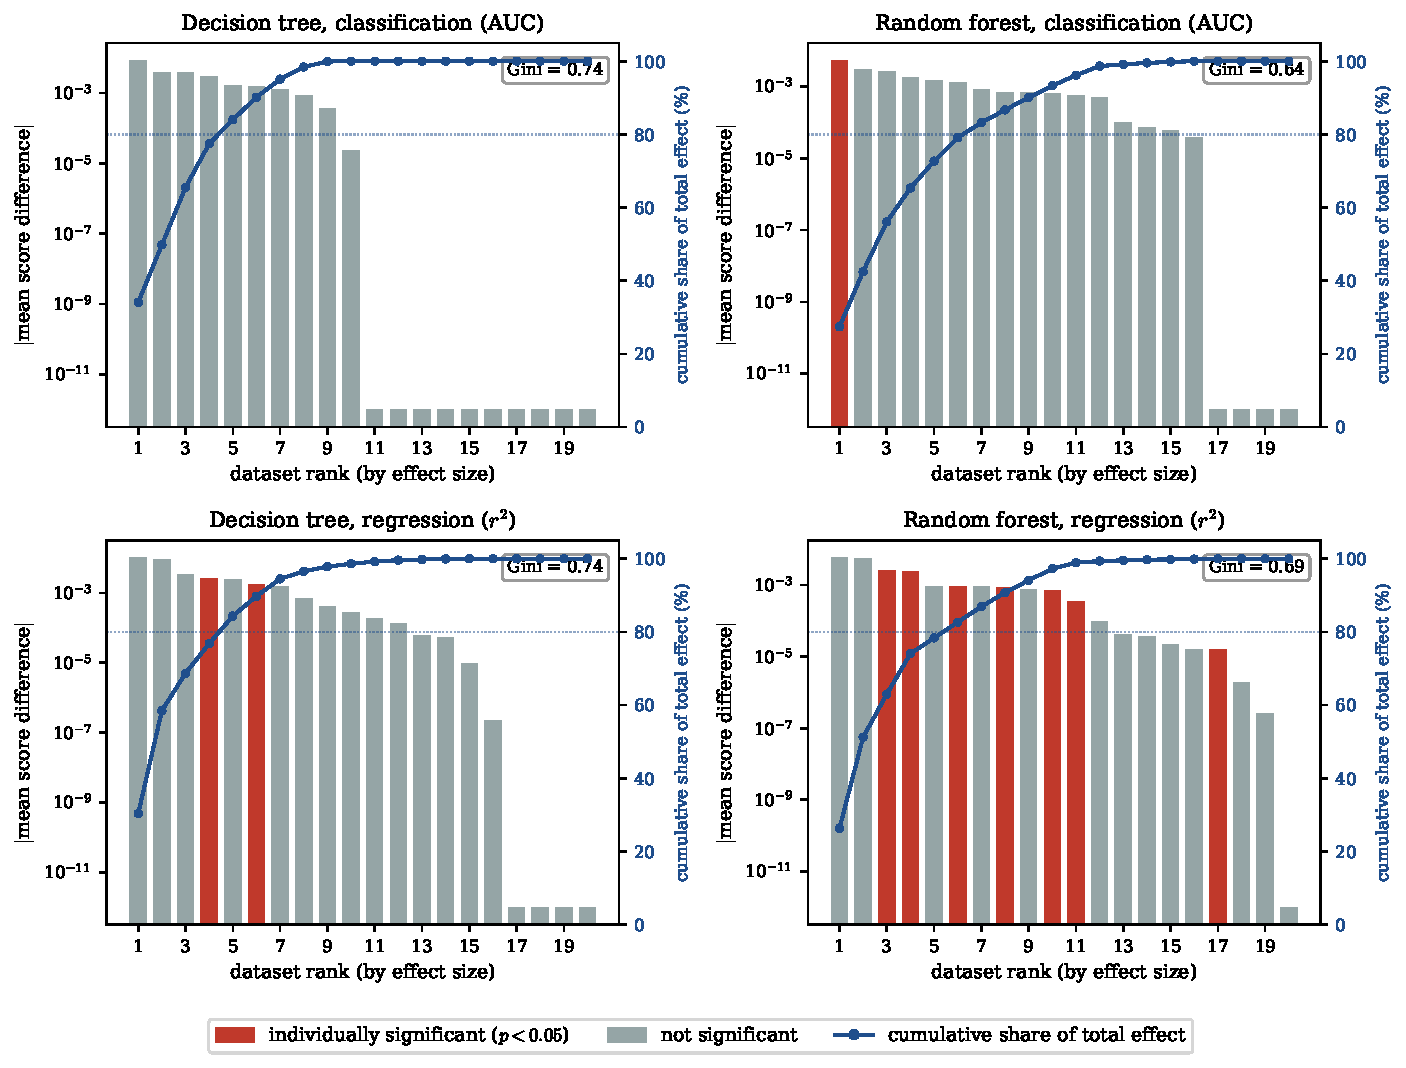
\includegraphics[width=0.8\textwidth]{heavytail_v6.pdf}
  \caption{Rank-ordered magnitude of the mean score difference between the proposed averaging method and $\text{worst}(\leq,<)$, across the 20-dataset pool of each estimator/problem-type combination (bars, log scale), together with the cumulative share of the total summed effect captured by the $k$ most-affected datasets (line, right axis) and the Gini coefficient of the effect-size distribution. The effect is heavy-tailed: a small minority of datasets carry most of the total effect -- the cumulative-share curve clears 80\% within the first 5--7 of 20 datasets in every panel -- and it is these datasets -- not a uniformly small effect across the whole pool -- that drive both the individually significant cells of Table \ref{tab:proof} and the cross-dataset meta-analysis of Section \ref{sec:meta}.}
  \label{fig:heavytail}
\end{figure*}


\subsubsection{Performance restricted to affected instances}
\label{sec:biased-instances}

The analyses above characterize the bias at the level of nodes ($\rho$) and datasets (the heavy-tail effect). A natural, more direct question is which individual \emph{records} the bias can possibly affect, and how the two operators perform on exactly that subset -- since averaging over the vast majority of unaffected records is precisely what makes the aggregate effect look small in Table \ref{tab:proof}. We flag a test instance as \emph{hit} if, along its default ($\leq$) traversal path through the final fitted model, at least one visited node's threshold exactly equals the instance's value on the split feature (for a forest, hit in at least one tree); such a node is, by construction, the only point at which $\leq$ and $<$ can possibly route the instance differently. We reuse the identical nested per-split procedure and final fitted models of Section \ref{sec:tests-model} to obtain this flag, rather than a separate pipeline, and confirmed as a correctness check that $\leq$ and $<$ predictions are bit-identical on every non-hit instance across all $80\times100$ outer splits evaluated.

Table \ref{tab:biasedinstance} summarizes the results. Hit rates for decision trees are close to zero (median $0.06\%$ for classification, $0.43\%$ for regression): the aggressive depth regularization that decision trees receive in model selection means a test record almost never lands exactly on a threshold gap. Random forests are entirely different -- median hit rates of $10.4\%$ (classification) and $26.0\%$ (regression), reaching as high as $85.8\%$ and $97.8\%$ for individual datasets -- consistent with the lighter regularization and larger $\rho$ already reported for random forest trees (Section \ref{sec:integrate}). The hit rate is also a substantially better predictor of a dataset's heavy-tail effect size (Figure \ref{fig:heavytail}) than $\rho$ was: the Spearman correlation between hit rate and $|\text{avg} - \text{worst}(\leq,<)|$ reaches $0.86$ for decision tree classification, the one combination where $\rho$'s correlation with effect size was weakest (Section \ref{sec:tests-quant}); an instance-level measure of exposure, it turns out, explains which datasets are affected considerably better than a node-level one does.

For random forests, where hit subsets are large enough to trust (median $323$ pooled hit instances for classification, $1271$ for regression, across the $100$ splits), restricting evaluation to hit instances reveals an averaging benefit $5.8\times$ larger for classification and $7.4\times$ larger for regression than on the full test set. Restricting the paper's own corrected significance test to splits with at least $5$ hit instances tells the same story with proper inference rather than a pooled point estimate: for random forest regression, $17$ of $20$ datasets have enough hit instances to test, and the averaging method wins on all $17$ (sign-test $p=1.5\times10^{-5}$, Fisher $p=1.5\times10^{-7}$) -- a combined $p$-value \emph{stronger} than the full-data meta-analysis of Section \ref{sec:meta} despite using less data per dataset, because the signal is no longer diluted by unaffected instances. Random forest classification shows the same pattern, with the familiar Fisher-dilution caveat (Section \ref{sec:select}); decision trees essentially never have enough hit instances per split to run this test at all (Table \ref{tab:biasedinstance}) -- itself confirming that depth regularization makes the bias practically unreachable at prediction time for almost every dataset in the pool.

\begin{table}[tbp]
  \caption{Performance restricted to instances that hit a biased node (Section \ref{sec:biased-instances}). \emph{median hit rate} is the fraction of test instances, pooled across the $R=100$ splits, that hit a biased node; $r_S(\text{hit}, \text{effect})$ is the Spearman correlation, across the 20-dataset pool, between per-dataset hit rate and the heavy-tail effect size of Figure \ref{fig:heavytail}; $n$ qualified counts datasets with at least one outer split containing $\ge 5$ hit instances, the minimum required to compute a per-split score restricted to the hit subset; wins/losses, the sign-test $p$-value, Fisher $p$, and $n_{sig}$ are computed exactly as in Table \ref{tab:meta}, restricted to hit instances within qualifying datasets/splits. A dash indicates fewer than two qualifying datasets, too few for a meaningful test.}
  \label{tab:biasedinstance}
  \centering
    \begin{footnotesize}
      \resizebox{\linewidth}{!}{\begin{tabular}{l@{\hspace{4pt}}r@{\hspace{4pt}}r@{\hspace{4pt}}r@{\hspace{4pt}}r@{\hspace{4pt}}r@{\hspace{4pt}}r@{\hspace{4pt}}r}
\toprule
estimator & hit rate & $r_S$(hit,\ eff.) & $n$ qual. & wins/losses & sign $p$ & Fisher $p$ & $n_{sig}$ \\
\midrule
DT classif. & 0.06\% & 0.86 & 0/20 & -- & -- & -- & -- \\
RF classif. & 10.45\% & 0.34 & 13/20 & 10/0 & 2.0e-03 & 7.3e-01 & 1 \\
DT regr. & 0.43\% & 0.56 & 1/20 & -- & -- & -- & -- \\
RF regr. & 26.03\% & 0.66 & 17/20 & 17/0 & 1.5e-05 & 1.5e-07 & 5 \\
\bottomrule
\end{tabular}
}
    \end{footnotesize}
\end{table}


\subsubsection{Operator selection as a compared method}
\label{sec:select}

Section \ref{sec:hyper} argued, on theoretical grounds, that cross-validating the operator is not useful. We test this directly: within each outer split's training portion, after selecting $\beta$ (Section \ref{sec:tests-model}), we score $\leq$ against $<$ on the same inner-validation folds and pick whichever scored higher, comparing this nested selection procedure against averaging as a fourth, explicit alternative. Unlike an in-sample proxy -- which, for a single decision tree, provably cannot distinguish the two operators at all, since every threshold is by construction the midpoint of a training-value gap -- this selection is scored on data the fitted model has not seen, giving it a genuine, if fold-limited, opportunity to find a real signal.

\begin{table}[tbp]
  \caption{Cross-dataset meta-analysis of the nested-CV operator-selection procedure of Section \ref{sec:tests-model} against the proposed averaging method, across the 20-dataset pool for each of the four estimator/problem type combinations. \emph{wins/losses} counts, among datasets with a nonzero mean difference, how many favor the selection procedure versus the averaging method (datasets tied at exactly zero, see below, are excluded from this count but not from Fisher's combination); a negative skew (more losses than wins) means the averaging method beats operator selection more often than the reverse. The sign-test $p$-value tests the wins/losses split against the 50/50 null; Fisher $p$ combines all 20 datasets' corrected $p$-values (Section \ref{sec:tests-testing}) into a single statistic; $n_{sig}$ counts datasets individually significant under the corrected test alone.}
  \label{tab:meta-select}
  \centering
    \begin{small}
      \begin{tabular}{l@{\hspace{6pt}}r@{\hspace{6pt}}r@{\hspace{6pt}}r@{\hspace{6pt}}r}
\toprule
estimator & wins/losses & sign-test $p$ & Fisher $p$ & $n_{sig}$ \\
\midrule
DT classif. & 2/9 & 6.5e-02 & 1 & 0 \\
RF classif. & 7/11 & 4.8e-01 & 1 & 0 \\
DT regr. & 3/13 & 2.1e-02 & 1 & 0 \\
RF regr. & 4/15 & 1.9e-02 & 1 & 0 \\
\bottomrule
\end{tabular}

    \end{small}
\end{table}

Table \ref{tab:meta-select} reports this cross-dataset meta-analysis, using the same sign test and Fisher's method as every other cross-dataset aggregation in this section. The result is unambiguous: \emph{selection does not outperform averaging, and where the sign test reaches significance, averaging wins}, for all four estimator/problem-type combinations (2/9, 7/11, 3/13, 4/15 for DT classif., RF classif., DT regr., RF regr., respectively), reaching significance for both regression estimators ($p=0.021$/$p=0.019$). This is a stronger result than an in-sample proxy could give, since the selection has genuine held-out signal available to it, yet still does not surpass simple averaging. Fisher's combined $p$-value, however, stays large throughout: datasets with essentially no lattice-aligned thresholds produce a mean difference of exactly zero, contributing neither a win nor a loss to the sign test but still a corrected $p$-value of 1 to Fisher's combination -- correctly diluting rather than inflating it. It is therefore the sign test, not Fisher's method, that carries the relevant evidence here.

For completeness, we also computed a hit-rate diagnostic: restricted to splits where the two operators genuinely differ on the held-out test portion, how often does the selected operator match the one that turns out better? Table \ref{tab:hitrate} reports the results, and they are consistent: the mean hit rate stays within 0.39--0.53 across all estimator types, with the sign test never approaching significance ($p \ge 0.45$). Even with genuine held-out signal, the nested-CV procedure carries essentially no information about which operator actually performs better -- explaining why it fails to outperform averaging in Table \ref{tab:meta-select}.

\begin{table}[tbp]
  \caption{Hit-rate diagnostic for the nested-CV operator-selection procedure of Section \ref{sec:tests-model}: restricted to splits where $\leq$ and $<$ genuinely differ on the held-out test portion, how often does the selected operator match the one that turns out better? $n$ datasets counts how many of the 20 datasets in the pool had at least 2 such splits (needed to compute a meaningful rate).}
  \label{tab:hitrate}
  \centering
    \begin{scriptsize}
      \begin{tabular}{l@{\hspace{6pt}}r@{\hspace{6pt}}r@{\hspace{6pt}}r@{\hspace{6pt}}r}
\toprule
estimator & $n$ datasets & mean hit rate & wins/losses vs.\ 0.5 & sign-test $p$ \\
\midrule
DT classif. & 9 & 0.394 & 2/5 & 4.5e-01 \\
RF classif. & 16 & 0.419 & 6/9 & 6.1e-01 \\
DT regr. & 14 & 0.464 & 7/6 & 1 \\
RF regr. & 19 & 0.530 & 9/8 & 1 \\
\bottomrule
\end{tabular}

    \end{scriptsize}
\end{table}


\subsubsection{Evaluation of the proposed method}
\label{sec:tests-proposed}

Having established the presence and heavy-tailed nature of the bias, we now turn to evaluating the proposed averaging method directly against the individual conditioning operators, using the $auc_{avg}$/$r^2_{avg}$ and $p_{avg}$ columns of Table \ref{tab:proof}.

As established in Section \ref{sec:proposed}, the proposed method's primary goal is to eliminate the risk of using a conditioning with a detrimental effect on performance. Using the same repeated holdout splits and corrected test as throughout this section, we compare the averaged prediction against $\text{worst}(\leq,<)$, the operator with the lower mean score on that dataset -- what a practitioner using the corresponding default implementation might unknowingly be exposed to. As Table \ref{tab:proof} shows, individually significant improvements are comparatively rare (0/20 for decision tree classification, 1 for random forest classification, 2 for decision tree regression, 7 for random forest regression), most consistent for random forest regression, and never in the opposite direction -- we did not observe a single dataset where the proposed method was significantly outperformed. As with the presence of the bias itself, this dataset-by-dataset view is necessary but not sufficient; the cross-dataset meta-analysis below is the primary evidence for the paper's central claim.

\label{sec:meta}
The per-dataset tests above and in Section \ref{sec:tests-quant} are individually often underpowered for an effect of this size -- a limitation of the test's conservatism, not evidence the effect is absent. We therefore aggregate evidence across the 20-dataset pool using the same two tools as Section \ref{sec:select}: a sign test against the 50/50 null, and Fisher's method combining all 20 datasets' corrected $p$-values, subject to the same tied-dataset dilution described there.

\begin{table}[tbp]
  \caption{Cross-dataset meta-analysis of the proposed averaging method against $\text{worst}(\leq,<)$, across the 20-dataset pool for each of the four estimator/problem type combinations. \emph{wins/losses} counts, among datasets with a nonzero mean score difference, how many favor the averaging method versus the reverse (datasets tied at exactly zero, see above, are excluded from this count but not from Fisher's combination); the sign-test $p$-value tests this split against the 50/50 null; Fisher $p$ combines all 20 datasets' corrected $p$-values (Section \ref{sec:tests-testing}) into a single statistic; $n_{sig}$ counts datasets individually significant under the corrected test alone. For $\leq$ vs.\ $<$ (not tabulated), the sign test never approaches significance for any estimator (all $p>0.16$), confirming, on real data, the same null result found under the idealized synthetic experiment of Section \ref{sec:synthetic}.}
  \label{tab:meta}
  \centering
    \begin{small}
      \begin{tabular}{l@{\hspace{6pt}}r@{\hspace{6pt}}r@{\hspace{6pt}}r@{\hspace{6pt}}r}
\toprule
estimator & wins/losses & sign-test $p$ & Fisher $p$ & $n_{sig}$ \\
\midrule
DT classif. & 10/0 & 2.0e-03 & 1 & 0 \\
RF classif. & 18/1 & 7.6e-05 & 8.8e-01 & 1 \\
DT regr. & 16/0 & 3.1e-05 & 4.9e-01 & 2 \\
RF regr. & 19/0 & 3.8e-06 & 7.2e-08 & 7 \\
\bottomrule
\end{tabular}

    \end{small}
\end{table}

Table \ref{tab:meta} presents this analysis. Two patterns stand out. First, the averaging method essentially never loses the sign test: it improves on far more datasets than it hurts for every estimator (10/0, 18/1, 16/0, 19/0 for DT classif., RF classif., DT regr., RF regr.), significant in every case ($p \le 2\times10^{-3}$). Second, the evidence is strongest for random forest regression: 7 of 20 datasets are individually significant, and Fisher's combined $p$-value reaches $7.2\times10^{-8}$. For the other three estimators, the sign test is decisively significant despite Fisher's $p$-value staying large (down to $4.9\times10^{-1}$ for decision tree regression) -- the same tied-dataset dilution discussed in Section \ref{sec:select}. We read the two statistics together: the sign test shows the direction is essentially never wrong, while Fisher's method shows how much of that direction survives the test's conservatism once diluted by unaffected datasets -- and for random forest regression, both agree emphatically.

For completeness, we ran the identical meta-analysis for $\leq$ versus $<$ individually (omitted from Table \ref{tab:meta} for space; full results in the code repository): the sign test never rejects the 50/50 null for any estimator (all $p > 0.16$), reinforcing Section \ref{sec:hyper}'s conclusion that only the averaging method shows a robust, aggregate advantage.


\section{Summary and Conclusions}
\label{sec:summary}

Decision trees and random forests are among the most commonly used supervised learning techniques, with popular implementations \citep{sklearn, tree} built on CART-type binary decision trees. This paper investigates two implicit modeling choices in such implementations: using the mid-point between observations as threshold ($t$), and conditioning in the form $x\leq t$ or $x<t$.

In Section \ref{sec:problem}, we showed that although conditioning has a negligible effect on continuous features, it can interfere with thresholds and impact predictions when features take values from equidistant domains -- a common situation in practice (Section \ref{sec:tests-datasets}, Table \ref{tab:datasets}). We refer to this variation as the \emph{conditioning bias}.

In Section \ref{sec:proposed}, we proposed eliminating the bias by integrating out the dependence on conditioning. Subsection \ref{sec:hyper} argued, and Section \ref{sec:tests} confirmed empirically, that the operator cannot be usefully cross-validated, since no operator is reliably better to begin with. Subsection \ref{sec:integrate} discussed the computational and interpretational aspects of integrating out the bias, and gave a direct, measured explanation for why bootstrap aggregation in random forests does not do this automatically -- with the added finding that elimination incurs no additional computational cost for random forests. Finally, subsection \ref{sec:equiv} showed how mirroring trees (or inducing trees from mirrored feature vectors) enables predictions under the non-default conditioning of an implementation without custom prediction engines.

In Section \ref{sec:tests}, we conducted an extensive evaluation on 40 classification and regression datasets under a fully nested cross-validation design and a corrected resampled $t$-test that avoids the anti-conservative bias of naive testing on pooled, non-independent repeated-CV folds. We complemented per-dataset testing with a cross-dataset meta-analysis, a direct comparison against a properly nested operator-selection procedure, and an independent synthetic experiment needing no such correction at all. The resulting picture is conservative but honest: we do not claim any specific operator is reliably detrimental on a given dataset, nor that cross-validation can reliably identify one -- our evidence, gathered four independent ways, argues against such claims. What we do show, robustly, and culminating in a cross-dataset combined $p$-value as low as $7\times10^{-8}$ for random forest regression (Section \ref{sec:meta}), is that the proposed averaging technique reliably outperforms the worse-performing operator, and does so at least as well as a genuine operator-selection procedure given every opportunity, short of leakage, to find real signal (Section \ref{sec:select}).

A further finding sharpens why this matters in practice: the effect is heavy-tailed, not uniformly small (Section \ref{sec:tests-quant}, Figure \ref{fig:heavytail}). For most datasets in our pool the bias is genuinely negligible, which is precisely why individual-dataset significance testing is so often underpowered; but for a minority -- those with an unusually high proportion of lattice-aligned nodes -- the effect is substantial, in one case nearly three orders of magnitude above the pool's typical case, and it is these datasets that drive essentially all of the individually significant results we observe. Crucially, whether a given dataset falls into the negligible bulk or the substantial tail cannot be determined without carrying out this paper's analysis on it directly. Restricting evaluation to exactly the records the bias can touch (Section \ref{sec:biased-instances}) confirms this is not a dilution artifact: for random forests, the averaging method's advantage there is stronger, not weaker, than in the full-population meta-analysis. Given that the technique is free for random forests and only doubles prediction time for single decision trees, this heavy-tailed, unpredictable risk profile is exactly the situation in which such a low-cost safeguard is worth adopting unconditionally -- the cost is small and uniform, while the protection it buys against the unpredictable, occasionally substantial tail case is what actually matters. We therefore conclude that it constitutes a low-risk, and for random forests a free-lunch, improvement worth adopting regardless of whether the bias happens to be individually detectable on any particular dataset at hand.

Finally, we mention that the implementation of the entire analysis is available at the GitHub repository \url{https://github.com/gykovacs/conditioning_bias}.

\section*{Acknowledgements}

This work was developed within the scope of the project
i3N, UIDB/50025/2020 and UIDP/50025/2020, financed by
national funds through the FCT/MEC-Portuguese Foundation for Science and Technology. G.T. was supported by FCT
Grant No. CEECIND/03838/2017.

\appendix

    \section{Sample data}
    \label{sec:sample}

    \begin{table}[tbp]
        \caption{The sample data the example trees can be inferred from.}
        \label{tab:sample}
    \centering
      \begin{tabular}{rrrr}
          \toprule
          self-employed & income (k) & dependents & target \\
          \midrule
          0 & 80 & 1 & 1 \\
          0 & 60 & 3 & 1 \\
          0 & 80 & 1 & 0 \\
          1 & 50 & 2 & 0 \\
          1 & 50 & 4 & 1 \\
          1 & 70 & 4 & 0 \\
          \bottomrule
        \end{tabular}
    \end{table}

    The decision tree in Figure \ref{fig:dt} can be inferred from the data shared in Table \ref{tab:sample}.
    The target label encodes if the applicant will default (1) or pay back (0). The tree is induced by the \emph{sklearn} (version 1.5.1) \citep{sklearn} decision tree classifier using the random seed 5.

\bibliographystyle{elsarticle-harv}
\bibliography{refs}% common bib file

\end{document}
